\documentclass{beamer}\usepackage[]{graphicx}\usepackage[]{color}
%% maxwidth is the original width if it is less than linewidth
%% otherwise use linewidth (to make sure the graphics do not exceed the margin)
\makeatletter
\def\maxwidth{ %
  \ifdim\Gin@nat@width>\linewidth
    \linewidth
  \else
    \Gin@nat@width
  \fi
}
\makeatother

\definecolor{fgcolor}{rgb}{0.345, 0.345, 0.345}
\newcommand{\hlnum}[1]{\textcolor[rgb]{0.686,0.059,0.569}{#1}}%
\newcommand{\hlstr}[1]{\textcolor[rgb]{0.192,0.494,0.8}{#1}}%
\newcommand{\hlcom}[1]{\textcolor[rgb]{0.678,0.584,0.686}{\textit{#1}}}%
\newcommand{\hlopt}[1]{\textcolor[rgb]{0,0,0}{#1}}%
\newcommand{\hlstd}[1]{\textcolor[rgb]{0.345,0.345,0.345}{#1}}%
\newcommand{\hlkwa}[1]{\textcolor[rgb]{0.161,0.373,0.58}{\textbf{#1}}}%
\newcommand{\hlkwb}[1]{\textcolor[rgb]{0.69,0.353,0.396}{#1}}%
\newcommand{\hlkwc}[1]{\textcolor[rgb]{0.333,0.667,0.333}{#1}}%
\newcommand{\hlkwd}[1]{\textcolor[rgb]{0.737,0.353,0.396}{\textbf{#1}}}%

\usepackage{framed}
\makeatletter
\newenvironment{kframe}{%
 \def\at@end@of@kframe{}%
 \ifinner\ifhmode%
  \def\at@end@of@kframe{\end{minipage}}%
  \begin{minipage}{\columnwidth}%
 \fi\fi%
 \def\FrameCommand##1{\hskip\@totalleftmargin \hskip-\fboxsep
 \colorbox{shadecolor}{##1}\hskip-\fboxsep
     % There is no \\@totalrightmargin, so:
     \hskip-\linewidth \hskip-\@totalleftmargin \hskip\columnwidth}%
 \MakeFramed {\advance\hsize-\width
   \@totalleftmargin\z@ \linewidth\hsize
   \@setminipage}}%
 {\par\unskip\endMakeFramed%
 \at@end@of@kframe}
\makeatother

\definecolor{shadecolor}{rgb}{.97, .97, .97}
\definecolor{messagecolor}{rgb}{0, 0, 0}
\definecolor{warningcolor}{rgb}{1, 0, 1}
\definecolor{errorcolor}{rgb}{1, 0, 0}
\newenvironment{knitrout}{}{} % an empty environment to be redefined in TeX

\usepackage{alltt}
\usetheme{default}
%\usetheme{Malmoe}

\title[EC999: Quantitative Text Analysis]{EC999: Part of Speech Tagging} \def\newblock{\hskip .11em plus .33em minus .07em}


\def\Tiny{\fontsize{10pt}{10pt}\selectfont}
\def\smaller{\fontsize{8pt}{8pt}\selectfont}

\institute[Warwick]{University of Chicago \& University of Warwick}
\author[Thiemo Fetzer]{Thiemo Fetzer}

 \date{\today}

\usepackage{natbib}
\usepackage{amsmath}
\usepackage{hyperref}
\usepackage{graphicx}
\usepackage{graphics}

\usepackage{amsfonts}
\usepackage{amssymb}
\usepackage{pdfpages}
\usepackage{natbib}
\usepackage{hyperref}
%\usepackage{enumitem}
 \usepackage{pgffor}
\usepackage{booktabs,caption,fixltx2e}
\usepackage[flushleft]{threeparttable}
\usepackage{verbatim} 
\usepackage{cancel}
\newcommand\xxcancel[1]{\xcancel{#1}\vphantom{#1}}

\usepackage{mathtools,xparse}

\newenvironment{Description}
               {\list{}{\labelwidth=0pt \itemindent-\leftmargin
                        \let\makelabel\Descriptionlabel
                        % or whatever
               }}
               {\endlist}
\newcommand*\Descriptionlabel[1]{%
  \hspace\labelsep
  \normalfont%  reset current font setting
  \color{blue}\bfseries\sffamily% or whatever 
  #1}


\setbeamersize{text margin left = 16pt, text margin right = 16pt}
\newcommand{\code}[1]{\texttt{#1}}

\newenvironment<>{algorithm}[1][\undefined]{%
\begin{actionenv}#2%
\ifx#1\undefined%
   \def\insertblocktitle{Algorithm}%
\else%
   \def\insertblocktitle{Algorithm ({\em#1})}%
\fi%
\par%
\mode<presentation>{%
  \setbeamercolor{block title}{fg=white,bg=yellow!50!black}
  \setbeamercolor{block body}{fg=black,bg=yellow!20}
}%
\usebeamertemplate{block begin}\em}
{\par\usebeamertemplate{block end}\end{actionenv}}


\newenvironment<>{assumption}[1][\undefined]{%
\begin{actionenv}#2%
\ifx#1\undefined%
   \def\insertblocktitle{Assumption}%
\else%
   \def\insertblocktitle{Assumption ({\em#1})}%
\fi%
\par%
\mode<presentation>{%
  \setbeamercolor{block title}{fg=white,bg=blue!50!black}
  \setbeamercolor{block body}{fg=black,bg=blue!20}
}%
\usebeamertemplate{block begin}\em}
{\par\usebeamertemplate{block end}\end{actionenv}}

%changing spacing between knitr code and output
\usepackage{etoolbox} 
\makeatletter 
\preto{\@verbatim}{\topsep=0pt \partopsep=0pt } 
\makeatother
\renewenvironment{knitrout}{\setlength{\topsep}{0mm}}{}
\IfFileExists{upquote.sty}{\usepackage{upquote}}{}
\begin{document}



\AtBeginSection[]
{
 \begin{frame}<beamer>
 \frametitle{Plan}
 \tableofcontents[currentsection]
 \end{frame}
}
\maketitle
 

%%%%%%%%%%%%%%%%%%%%%%%%%%%%


%%%%%%%%%%%%%%%%%%%%%%%%%%%%%%%%%%%%%%%%%%%%%%%%%%%%%%%%%%
\begin{frame}[fragile]{Part of Speech Tagging}

Classical \emph{Part's of speech} are: nouns, verbs, pronouns, preopositions, adverbs, conjunctions, participles and articles. \smallskip

Part of spech (POS) tagging is an essential step in language processing that is very useful for a range of auxiliary tasks.

\begin{itemize}

\item dimensionality reduction (removing words)\smallskip

\item word sense disambiguation\smallskip

\item Named Entity Recognition \smallskip

\item information extraction 

\end{itemize}

$\Rightarrow$ we will introduce the formalization of common tools for POS tagging and introduce use pipelines in $R$. 
\end{frame}
%%%%%%%%%%%%%%%%%%%%%%%%%%%%%%%%%%%%%%%%%%%%%%%%%%%%%%%%%%%%%%%%%%%%%%%%%



%%%%%%%%%%%%%%%%%%%%%%%%%%%%%%%%%%%%%%%%%%%%%%%%%%%%%%%%%%
\begin{frame}[fragile]{Part of Speech Tagging}

Classical \emph{Part's of speech} are: nouns, verbs, pronouns, preopositions, adverbs, conjunctions, participles and articles. \smallskip

Part of spech (POS) tagging is an essential step in language processing that is very useful for a range of auxiliary tasks.

\begin{itemize}

\item dimensionality reduction (removing words)\smallskip

\item word sense disambiguation\smallskip

\item Named Entity Recognition \smallskip

\item information extraction 

\end{itemize}

$\Rightarrow$ we will introduce the formalization of common tools for POS tagging and introduce use pipelines in $R$. 
\end{frame}
%%%%%%%%%%%%%%%%%%%%%%%%%%%%%%%%%%%%%%%%%%%%%%%%%%%%%%%%%%%%%%%%%%%%%%%%%


%%%%%%%%%%%%%%%%%%%%%%%%%%%%%%%%%%%%%%%%%%%%%%%%%%%%%%%%%%
\begin{frame}[fragile]{Part of Speech Tagging}


\begin{center}
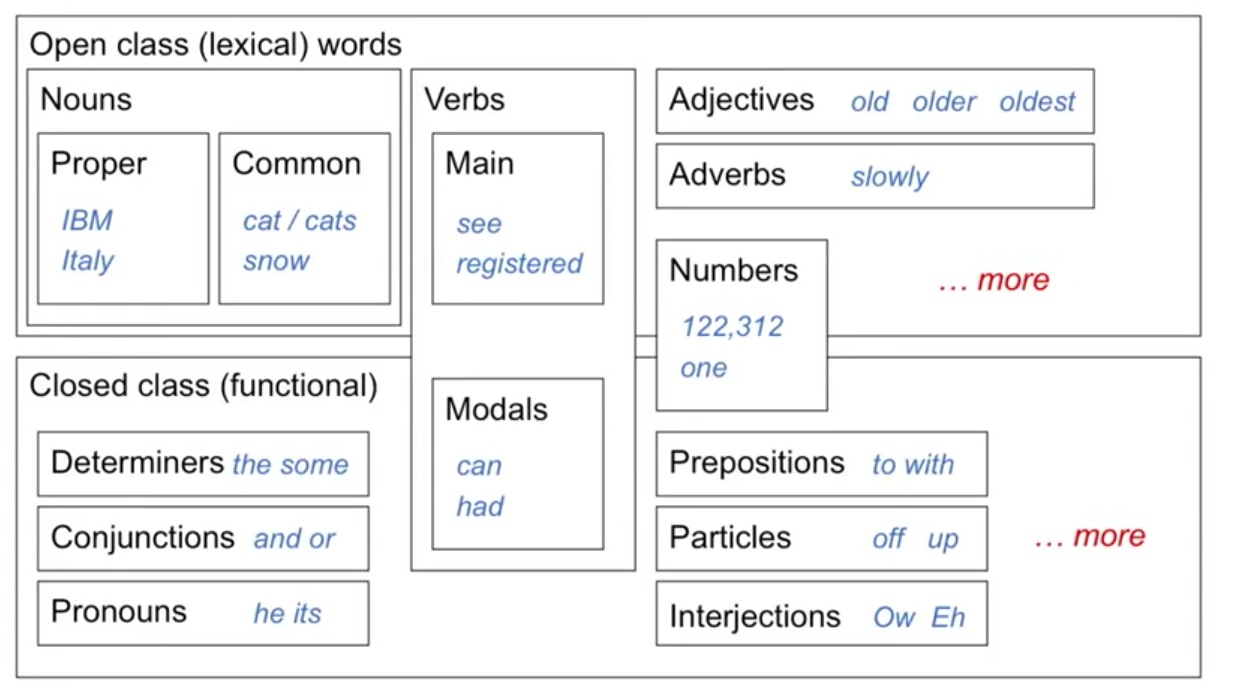
\includegraphics[scale=0.5]{figures/parts-of-speech.png}
\end{center}

\end{frame}
%%%%%%%%%%%%%%%%%%%%%%%%%%%%%%%%%%%%%%%%%%%%%%%%%%%%%%%%%%%%%%%%%%%%%%%%%



%%%%%%%%%%%%%%%%%%%%%%%%%%%%%%%%%%%%%%%%%%%%%%%%%%%%%%%%%%
\begin{frame}[fragile]{Open Versus Closed Class}

Typically two types of high level groups are defined

\begin{itemize}

\item \textbf{Closed class}: considered as closed as the set of closed class words hardly changes over time.
\begin{itemize} 

\item determiners: a, an, the 
\item pronouns: I, he, she, they
\item prepositions: over, under, near \smallskip
\end{itemize}

\item \textbf{Open class}: New entries into classes of all types, think of proper nouns becoming verbs - such as "Google" and "to google".
\end{itemize}

\end{frame}
%%%%%%%%%%%%%%%%%%%%%%%%%%%%%%%%%%%%%%%%%%%%%%%%%%%%%%%%%%%%%%%%%%%%%%%%%


%%%%%%%%%%%%%%%%%%%%%%%%%%%%%%%%%%%%%%%%%%%%%%%%%%%%%%%%%%
\begin{frame}[fragile]{Word Class Ambiguity makes this a challenging task}

Part of speech tagging is challenging as words can be members of multiple classes, depending on the \emph{context} of use.

\begin{itemize}

\item \code{get/VB off/IN my/PRP\$ \textbf{back/NN}}\smallskip

\item  \code{win/VB the/DT voters/NNS \textbf{back/RB}} \smallskip

\item \code{I/PRP promise/VBP to/TO back/VB the/DT bill/NN ./.}\smallskip

\end{itemize}

Part of speech tagging task is a relatively \emph{easy} task. For every word that has ambiguity, there is a constrained set of ambiguous tags to chose from. Most POS implementation work off the information contained by the word itself and on information contained by small \emph{windows} around the word.
\end{frame}
%%%%%%%%%%%%%%%%%%%%%%%%%%%%%%%%%%%%%%%%%%%%%%%%%%%%%%%%%%%%%%%%%%%%%%%%%




%%%%%%%%%%%%%%%%%%%%%%%%%%%%%%%%%%%%%%%%%%%%%%%%%%%%%%%%%%
\begin{frame}[fragile]{The Penn Treebank Part-of-Speech Tagset}

There are many lists of parts-of-speech, most modern language processing on English uses the 45-tag Penn Treebank tagset.
\begin{center}
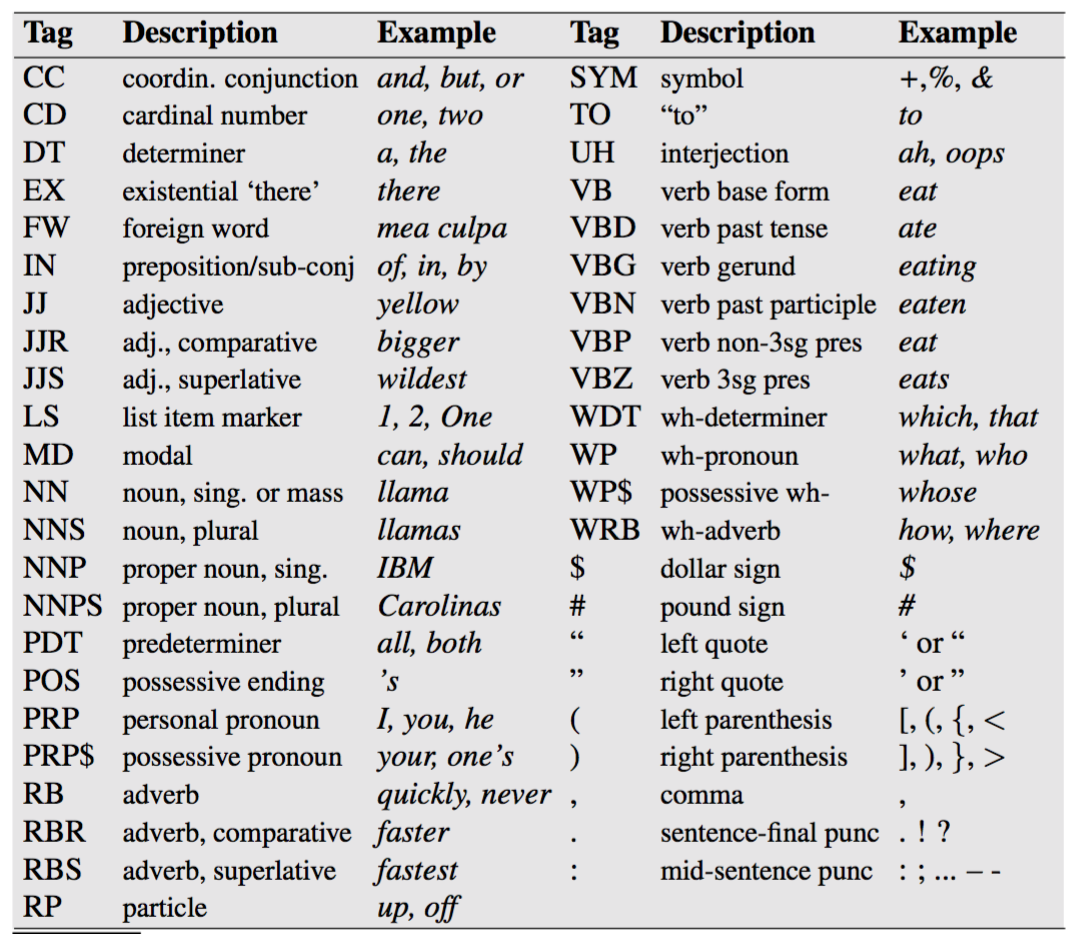
\includegraphics[scale=0.33]{figures/penn-treebank-pos.png}
\end{center}
There are other tagsets $T$ with anything between 8 to 1,200, but this is the most commonly used 
\end{frame}
%%%%%%%%%%%%%%%%%%%%%%%%%%%%%%%%%%%%%%%%%%%%%%%%%%%%%%%%%%%%%%%%%%%%%%%%%




%%%%%%%%%%%%%%%%%%%%%%%%%%%%%%%%%%%%%%%%%%%%%%%%%%%%%%%%%%
\begin{frame}[fragile]{A naive POS tagger}

The \emph{baseline} POS tagger uses a simple tag-allocation rule: assign a tag $t^* \in T$ to a word $w_j$ if 

$$ t^* = argmax P(t_i|w_j) $$

This tag allocation rule assigns the tag $t$ to a word $w_j$ that has the highest likelihood for that word. These conditional likelihoods can be estimated from some tagged \emph{training} data.\smallskip

It achieves surprising accuracy of around 90\%.\smallskip

Reason for surprising high accuracy is due to fact that a lot of \emph{stopwords} that make up the bulk of the quantity of tokens of text have mostly unambigous tags.

\end{frame}
%%%%%%%%%%%%%%%%%%%%%%%%%%%%%%%%%%%%%%%%%%%%%%%%%%%%%%%%%%%%%%%%%%%%%%%%%


%%%%%%%%%%%%%%%%%%%%%%%%%%%%%%%%%%%%%%%%%%%%%%%%%%%%%%%%%%
\begin{frame}[fragile]{Accuracy of Naive POS}

For example for the word \code{well}:

\begin{itemize}

\item \code{Get/VB well/RB soon/RB !/.}\smallskip

\item  \code{This/DT oil/NN well/NN is/VBZ profitable/JJ ./.} \smallskip

\end{itemize}

For the word \code{well}, a training corpus suggests

\begin{center}
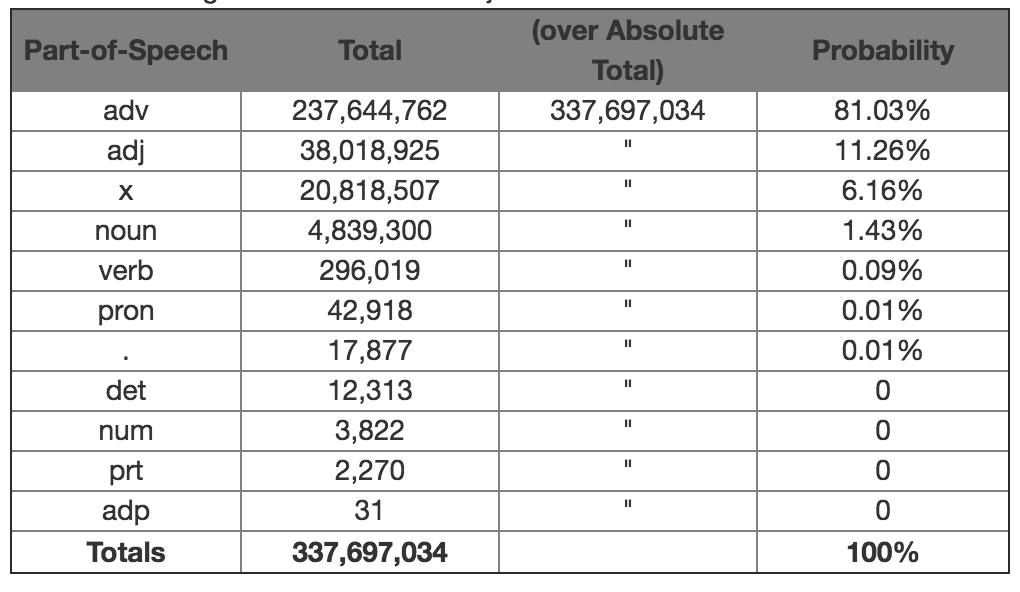
\includegraphics[scale=.3]{figures/well-pos.png}
\end{center}

This suggests that the naive model would suggest that the most likely class for the word is \code{RB} - adverb form.

\end{frame}
%%%%%%%%%%%%%%%%%%%%%%%%%%%%%%%%%%%%%%%%%%%%%%%%%%%%%%%%%%%%%%%%%%%%%%%%%



%%%%%%%%%%%%%%%%%%%%%%%%%%%%%%%%%%%%%%%%%%%%%%%%%%%%%%%%%%
\begin{frame}[fragile]{A (shallow) deep dive: Hidden Markov Models}

One direction to improve on baseline POS tagger is to use information contained in structure around a word. So suppose you have a word sequence $w_1, ..., w_n$ (like a sentence), then the optimization problem that you want to solve is to assign a sequence of tags $t_1, ..., t_n$ to these words, that maximizes the probability

$$ (t_1,...,t_n)* = argmax P((t_1,...,t_n) | (w_1,...,w_n)) $$

The underlying (hidden) true states of the world is the correct tag sequence $t_1,...,t_n$.

It is impractical (impossible) to estimate $P((t_1,...,t_n) | (w_1,...,w_n)) $ directly from training data due to the sparsity. So we employ a simplifying assumption.

\end{frame}
%%%%%%%%%%%%%%%%%%%%%%%%%%%%%%%%%%%%%%%%%%%%%%%%%%%%%%%%%%%%%%%%%%%%%%%%%


%%%%%%%%%%%%%%%%%%%%%%%%%%%%%%%%%%%%%%%%%%%%%%%%%%%%%%%%%%
\begin{frame}[fragile]{A (shallow) deep dive: Hidden Markov Models}

We can apply \emph{Bayes Rule}, so the optimization problem becomes

$$ (t_1,...,t_n)^* = argmax \frac{P((w_1,...,w_n) | (t_1,...,t_n)) P(t_1, ..., t_n)}{P((w_1,..., w_n))} $$

This optimization problem is equivalent to solving [why?]

$$ (t_1,...,t_n)^* = argmax P((w_1,...,w_n) | (t_1,...,t_n)) P(t_1, ..., t_n) $$
 
\end{frame}
%%%%%%%%%%%%%%%%%%%%%%%%%%%%%%%%%%%%%%%%%%%%%%%%%%%%%%%%%%%%%%%%%%%%%%%%%



%%%%%%%%%%%%%%%%%%%%%%%%%%%%%%%%%%%%%%%%%%%%%%%%%%%%%%%%%%
\begin{frame}[fragile]{A (shallow) deep dive: Hidden Markov Models}

For Hidden Markov POS models, we make two additional assumptions

$$P((w_1,...,w_n)) = \prod_{i=1}^n P(w_i|t_i)$$

and

$$P((t_1,...,t_n)) = \prod_{i=1}^n P(t_i | t_{i-1})$$

This allows us to rewrite the optimization problem as

$$ (t_1,...,t_n)^* = argmax \prod_{i=1}^n{P(w_i|t_i) P(t_i|t_{i-1})} $$

\end{frame}
%%%%%%%%%%%%%%%%%%%%%%%%%%%%%%%%%%%%%%%%%%%%%%%%%%%%%%%%%%%%%%%%%%%%%%%%%


%%%%%%%%%%%%%%%%%%%%%%%%%%%%%%%%%%%%%%%%%%%%%%%%%%%%%%%%%%
\begin{frame}[fragile]{An example: Hidden Markov Models}

Consider the sentence \smallskip

\code{Janet will back the bill} \bigskip

which is correctly tagged as  \smallskip

\code{Janet/NNP will/MD back/VB the/DT bill/NN} \bigskip

We obtain the following information from a tagged training corpus.
\end{frame}
%%%%%%%%%%%%%%%%%%%%%%%%%%%%%%%%%%%%%%%%%%%%%%%%%%%%%%%%%%%%%%%%%%%%%%%%%


%%%%%%%%%%%%%%%%%%%%%%%%%%%%%%%%%%%%%%%%%%%%%%%%%%%%%%%%%%
\begin{frame}[fragile]{An example: Hidden Markov Models}


\begin{center}
\includegraphics[scale=0.5]<1>{figures/jurafsky-example-pwt.png}
\includegraphics[scale=0.5]<2>{figures/jurafsky-example-t-t-1.png}
\end{center}

Displaying $P(w_i|t_i) $ and $P(t_i|t_{i-1})$.

\end{frame}
%%%%%%%%%%%%%%%%%%%%%%%%%%%%%%%%%%%%%%%%%%%%%%%%%%%%%%%%%%%%%%%%%%%%%%%%%

%%%%%%%%%%%%%%%%%%%%%%%%%%%%%%%%%%%%%%%%%%%%%%%%%%%%%%%%%%
\begin{frame}[fragile]{An example: Finding optimal path}

\begin{center}
\includegraphics[scale=0.4]<1>{figures/jurafsky-example-pwt.png}
\end{center}

\begin{itemize}

\item In the corpus, the word \code{Janet} only appears with tag \code{NNP}.\smallskip

\item the word \code{will} has three possible tags \code{MD, VB, NN}.\smallskip

\item The probability that a random word of type modal (MD) is the word \code{will} is 0.31 = $P(\text{\code{will}}|\text{\code{MD}})$ \smallskip

\end{itemize}

\end{frame}
%%%%%%%%%%%%%%%%%%%%%%%%%%%%%%%%%%%%%%%%%%%%%%%%%%%%%%%%%%%%%%%%%%%%%%%%%


%%%%%%%%%%%%%%%%%%%%%%%%%%%%%%%%%%%%%%%%%%%%%%%%%%%%%%%%%%
\begin{frame}[fragile]{An example: Finding optimal path}

\begin{center}
\includegraphics[scale=0.4]<1>{figures/jurafsky-example-t-t-1.png}
\end{center}

\begin{itemize}

\item Transition matrix presents estimated $P(t_i|t_{i-1})$.\smallskip

\item the row sums should add to 1 - they dont since not the whole tagset is displayed.\smallskip

\item $P(\text{\code{VB}}||\text{\code{MD}}) = 0.79$, probability that \code{MD} is followed by tag \code{VB}.

\end{itemize}

\end{frame}
%%%%%%%%%%%%%%%%%%%%%%%%%%%%%%%%%%%%%%%%%%%%%%%%%%%%%%%%%%%%%%%%%%%%%%%%%

%%%%%%%%%%%%%%%%%%%%%%%%%%%%%%%%%%%%%%%%%%%%%%%%%%%%%%%%%%
\begin{frame}[fragile]{An example: Finding optimal path}

\begin{center}
\includegraphics[scale=0.4]<1>{figures/jurafsky-example-path.png}
\end{center}

\begin{itemize}

\item The optimization problem can be modelled as an optimization problem on a \emph{directed path}. \smallskip

\item We want to find the path that has highest likelihood.\smallskip

\item Brute forcing - the computation of all possible values for $\prod_{i=1}^n{P(w_i|t_i) P(t_i|t_{i-1})}$ is computationaly extremely inefficient, and becomes infeasible very fast.\smallskip

\item \emph{Viterbi algorithm} is a dynamic programming algorithm that solves this program efficiently.
\end{itemize}

\end{frame}
%%%%%%%%%%%%%%%%%%%%%%%%%%%%%%%%%%%%%%%%%%%%%%%%%%%%%%%%%%%%%%%%%%%%%%%%%



%%%%%%%%%%%%%%%%%%%%%%%%%%%%%%%%%%%%%%%%%%%%%%%%%%%%%%%%%%
\begin{frame}[fragile]{Part of Speech Tagging in $R$}

In $R$ an easily accessible POS tagging tool that performs very well is accessible through the packages \code{OpenNLP}, which makes Apache's Open NLP platform accessible (\url{https://opennlp.apache.org/}).\bigskip

It is a bit slow and the Apache NLP package is memory intensive (requests around)\bigskip

Rather than working with a hidden markov model, its a maximum entropy classifier - which is just a fancy way of saying "logistic regression". We will introduce logistic regression for simple classification tasks.\smallskip
\end{frame}
%%%%%%%%%%%%%%%%%%%%%%%%%%%%%%%%%%%%%%%%%%%%%%%%%%%%%%%%%%%%%%%%%%%%%%%%%



%%%%%%%%%%%%%%%%%%%%%%%%%%%%%%%%%%%%%%%%%%%%%%%%%%%%%%%%%%
\begin{frame}[fragile]{Part of Speech Tagging in $R$}

We will work with a developmental extension called the \code{tagger} package. Speed is an issue with NLP pipelines, OpenNLP extension takes arund 0.1 seconds per ``sentence''.

\begin{knitrout}\tiny
\definecolor{shadecolor}{rgb}{0.969, 0.969, 0.969}\color{fgcolor}\begin{kframe}
\begin{alltt}
\hlkwd{library}\hlstd{(NLP)}
\hlkwd{library}\hlstd{(openNLP)}
\hlcom{# this is developmental, can be installed with the next two lines of code.}
\hlkwd{library}\hlstd{(tagger)}

\hlcom{## this installs 'pacman' which is a package to load developmental R extensions}
\hlkwa{if} \hlstd{(}\hlopt{!}\hlkwd{require}\hlstd{(}\hlstr{"pacman"}\hlstd{))} \hlkwd{install.packages}\hlstd{(}\hlstr{"pacman"}\hlstd{)}
\hlstd{pacman}\hlopt{::}\hlkwd{p_load_gh}\hlstd{(}\hlkwd{c}\hlstd{(}\hlstr{"trinker/termco"}\hlstd{,} \hlstr{"trinker/tagger"}\hlstd{))}

\hlstd{temp} \hlkwb{<-} \hlkwd{tag_pos}\hlstd{(}\hlstr{"Janet will back the bill"}\hlstd{)}

\hlstd{temp[[}\hlnum{1}\hlstd{]]}
\end{alltt}
\begin{verbatim}
##     NNP      MD      VB      DT      NN 
## "Janet"  "will"  "back"   "the"  "bill"
\end{verbatim}
\begin{alltt}
\hlkwd{data.frame}\hlstd{(}\hlkwc{tokens} \hlstd{= temp[[}\hlnum{1}\hlstd{]],} \hlkwc{tags} \hlstd{=} \hlkwd{names}\hlstd{(temp[[}\hlnum{1}\hlstd{]]))}
\end{alltt}
\begin{verbatim}
##     tokens tags
## NNP  Janet  NNP
## MD    will   MD
## VB    back   VB
## DT     the   DT
## NN    bill   NN
\end{verbatim}
\end{kframe}
\end{knitrout}
\end{frame}
%%%%%%%%%%%%%%%%%%%%%%%%%%%%%%%%%%%%%%%%%%%%%%%%%%%%%%%%%%%%%%%%%%%%%%%%%



%%%%%%%%%%%%%%%%%%%%%%%%%%%%%%%%%%%%%%%%%%%%%%%%%%%%%%%%%%
\begin{frame}[fragile]{Part of Speech Tagging in $R$}

\begin{knitrout}\tiny
\definecolor{shadecolor}{rgb}{0.969, 0.969, 0.969}\color{fgcolor}\begin{kframe}
\begin{alltt}
\hlkwd{data}\hlstd{(presidential_debates_2012)}

\hlstd{TAGGED} \hlkwb{<-} \hlkwd{tag_pos}\hlstd{(presidential_debates_2012}\hlopt{$}\hlstd{dialogue)}

\hlkwd{head}\hlstd{(TAGGED)}
\end{alltt}
\begin{verbatim}
## [[1]]
##            PRP             MD             VB             IN             RB             IN 
##           "We"          "'ll"         "talk"        "about" "specifically"        "about" 
##             NN             NN             IN             DT             NN              . 
##       "health"         "care"           "in"            "a"       "moment"            "." 
## 
## [[2]]
##         CC         WP        VBP        PRP         VB         DT         NN         NN 
##      "But"     "what"       "do"      "you"  "support"      "the"  "voucher"   "system" 
##          ,        NNP          . 
##        "," "Governor"        "?" 
## 
## [[3]]
##         WP        PRP        VBP        VBZ         DT         NN         IN         JJ 
##     "What"        "I"  "support"       "is"       "no"   "change"      "for"  "current" 
##        NNS         CC         IN        NNS         TO        NNP          . 
## "retirees"      "and"     "near" "retirees"       "to" "Medicare"        "." 
## 
## [[4]]
##          CC          DT          NN         VBZ         VBG          NN          CD 
##       "And"       "the" "president"  "supports"    "taking"    "dollar"     "seven" 
##          CD          CD          CD          IN          IN          DT          NN 
##   "hundred"   "sixteen"   "billion"       "out"        "of"      "that"   "program" 
##           . 
##         "." 
## 
## [[5]]
##         CC         WP         IN         DT        NNS          . 
##      "And"     "what"    "about"      "the" "vouchers"        "?" 
## 
## [[6]]
##       IN       DT      VBZ       DT      VBZ       NN       CD        . 
##     "So"   "that"     "'s"   "that"     "'s" "number"    "one"      "."
\end{verbatim}
\end{kframe}
\end{knitrout}
\end{frame}
%%%%%%%%%%%%%%%%%%%%%%%%%%%%%%%%%%%%%%%%%%%%%%%%%%%%%%%%%%%%%%%%%%%%%%%%%



%%%%%%%%%%%%%%%%%%%%%%%%%%%%%%%%%%%%%%%%%%%%%%%%%%%%%%%%%%
\begin{frame}[fragile]{Part of Speech Tagging in $R$}

\begin{knitrout}\tiny
\definecolor{shadecolor}{rgb}{0.969, 0.969, 0.969}\color{fgcolor}\begin{kframe}
\begin{alltt}
\hlkwd{plot}\hlstd{(TAGGED)}
\end{alltt}
\end{kframe}

{\centering 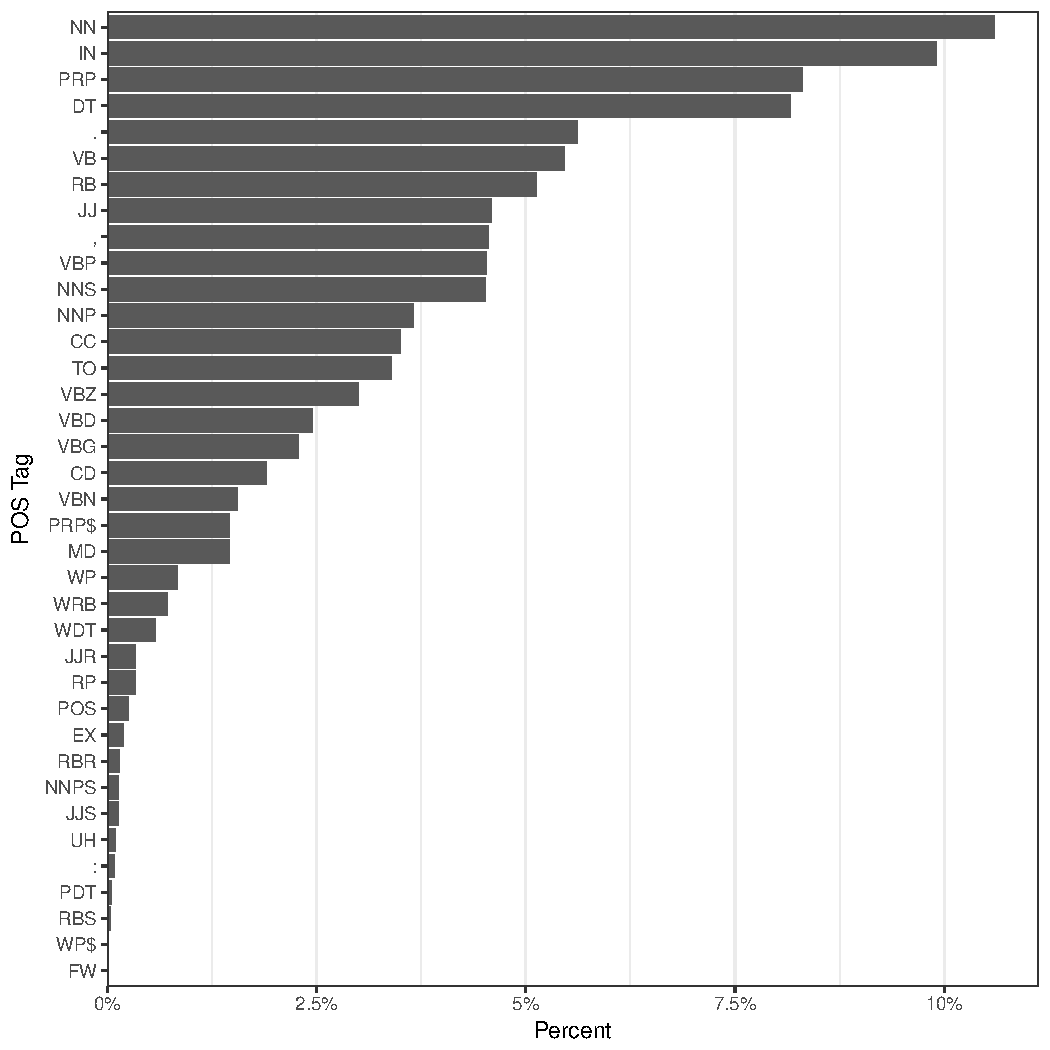
\includegraphics[width=3in]{figures/knitr-tagintodataframe-1} 

}



\end{knitrout}
\end{frame}
%%%%%%%%%%%%%%%%%%%%%%%%%%%%%%%%%%%%%%%%%%%%%%%%%%%%%%%%%%%%%%%%%%%%%%%%%




%%%%%%%%%%%%%%%%%%%%%%%%%%%%%%%%%%%%%%%%%%%%%%%%%%%%%%%%%%
\begin{frame}[fragile]{Going forward}

Part of Speech Tagging is an important and often neccesary task for NLP.\smallskip


We will make use of POS tags in a range of applications, so a basic understanding is needed.\smallskip



\end{frame}
%%%%%%%%%%%%%%%%%%%%%%%%%%%%%%%%%%%%%%%%%%%%%%%%%%%%%%%%%%%%%%%%%%%%%%%%%




\end{document}



%%%%%%%%%%%%%%%%%%%%%%%%%%%%%%%%%%%%%%%%%%%%%%%%%%%%%%%%%%
\begin{frame}[fragile]{Motivation}

How the world of work is changing or the Rise of the Machines\\smallskip

How can we measure structural change in the labor market?\smallskip

Conceputally, we can think of the impact of technological change on the labor market as having two distinct features.\smallskip

\begin{enumerate}

\item What do we do [things on]?\smallskip

\item How do we do things?\smallskip

\end{enumerate}

Measuring this amounts to understanding the relationship between \emph{verbs} and \emph{nouns}.



\end{frame}
%%%%%%%%%%%%%%%%%%%%%%%%%%%%%%%%%%%%%%%%%%%%%%%%%%%%%%%%%%%%%%%%%%%%%%%%%

